\documentclass{beamer}
\usepackage[latin1]{inputenc}
\usepackage{times}
\usepackage{tikz}
\usetheme{Luebeck}
%\usecolortheme{albatross}
\usepackage{amsmath,amsfonts,amsthm,amssymb}
\usepackage{setspace}
\usepackage{Tabbing}
\usepackage{fancyhdr}
\usepackage{lastpage}
\usepackage{extramarks}
\usepackage{chngpage}
\usepackage{soul,color}
\usepackage{graphicx,float,wrapfig}
\usepackage{xcolor}
\usepackage{listings}
\usepackage{float}
%\usepackage{subfloat}
\usepackage{subfig}
\usepackage{caption}
\usepackage{enumitem}
\usepackage{algpseudocode}

\definecolor{darkorange}{RGB}{240, 120, 0}
\definecolor{darkgreen}{RGB}{0, 128, 0}

\setbeamercolor{background canvas}{bg=white}
\setbeamercolor{frametitle}{fg=white, bg=darkorange}
\setbeamercolor{normal text}{bg=black,fg=black}
\setbeamercolor{structure}{bg=black, fg=darkorange}


\lstdefinestyle{customc}{
  belowcaptionskip=1\baselineskip,
  breaklines=true,
  frame=L,
  xleftmargin=\parindent,
  language=Python,
  showstringspaces=false,
  basicstyle=\footnotesize\ttfamily,
  keywordstyle=\bfseries\color{green!40!black},
  commentstyle=\itshape\color{purple!40!black},
  identifierstyle=\color{blue},
  stringstyle=\color{orange},
}

\lstdefinestyle{customc}{
  belowcaptionskip=1\baselineskip,
  breaklines=true,
  frame=L,
  xleftmargin=\parindent,
  language=Python,
  showstringspaces=false,
  basicstyle=\footnotesize\ttfamily,
  keywordstyle=\bfseries\color{green!40!black},
  commentstyle=\itshape\color{purple!40!black},
  identifierstyle=\color{blue},
  stringstyle=\color{orange},
}

\lstdefinestyle{customcsmall}{
  belowcaptionskip=1\baselineskip,
  breaklines=true,
  frame=L,
  xleftmargin=\parindent,
  language=Python,
  showstringspaces=false,
  basicstyle=\footnotesize\ttfamily,
  keywordstyle=\bfseries\color{green!24!black},
  commentstyle=\itshape\color{purple!24!black},
  identifierstyle=\color{blue},
  stringstyle=\color{orange},
}

\lstdefinestyle{customcsmall}{
  belowcaptionskip=1\baselineskip,
  breaklines=true,
  frame=L,
  xleftmargin=\parindent,
  language=Python,
  showstringspaces=false,
  basicstyle=\footnotesize\ttfamily,
  keywordstyle=\bfseries\color{green!24!black},
  commentstyle=\itshape\color{purple!24!black},
  identifierstyle=\color{blue},
  stringstyle=\color{orange},
}

\definecolor{MidGreen}{HTML}{00AA00}
\definecolor{MidYellow}{HTML}{AAAA00}

\title{Lecture 16: Discrete Fourier Transform, Spherical Harmonics}
\date{3/8/2016}
\institute{Chris Tralie, Duke University}
\author{COMPSCI/MATH 290-04}
\begin{document}

\frame{\titlepage}

\begin{frame}{Announcements}
\begin{itemize}[label=$\vartriangleright$]

\item Mini Assignment 3 due Sunday 3/13 11:55PM

\item Group Assignment 2 Out around Friday/Saturday, due Monday 3/28

\item Final projects assigned, first milestone due Wednesday 4/6

\item Midterm Thursday

\end{itemize}

\end{frame}

\begin{frame}{Table of Contents}
\begin{itemize}[label=$\blacktriangleright$]
	\item Numpy Squared Euclidean Distances
\end{itemize}
\begin{itemize}[label=$\vartriangleright$]
	\item Discrete Fourier Transform
\end{itemize}
\begin{itemize}[label=$\vartriangleright$]
	\item Spherical Harmonics
\end{itemize}
\end{frame}


\begin{frame}{Numpy: More Broadcasting}

\lstinputlisting[style=customc]{NumpyDemos/broadcasting.py}

\end{frame}


\begin{frame}{Squared Euclidean Distances in Matrix Form}
Notice that

\[ ||\vec{a} - \vec{b}||^2 = (\vec{a} - \vec{b}) \cdot (\vec{a}-\vec{b}) \]

\[ ||\vec{a} - \vec{b}||^2 = \vec{a} \cdot \vec{a} + \vec{b} \cdot \vec{b} - 2 \vec{a} \cdot \vec{b} \]

\uncover<2->{

Given points clouds $X$ and $Y$ expressed as $2 \times M$ and $2 \times N$ matrices, respectively, write code to compute an $M \times N$ matrix $D$ so that

\[ D[i, j] = ||X[:, i] - Y[:, j]||^2 \]

Without using any for loops!  Can use for ranking with Euclidean distance or D2 shape histograms, for example

}

\end{frame}


\begin{frame}{Brute Force Nearest Neighbors}

\lstinputlisting[style=customcsmall]{NumpyDemos/NearestNeighborBrute.py}

\end{frame}


\begin{frame}{Mini Assignment 3 API}

\lstinputlisting[style=customcsmall]{ICPAPI.py}

\end{frame}

\begin{frame}{Table of Contents}
\begin{itemize}[label=$\vartriangleright$]
	\item Numpy Squared Euclidean Distances
\end{itemize}
\begin{itemize}[label=$\blacktriangleright$]
	\item Discrete Fourier Transform
\end{itemize}
\begin{itemize}[label=$\vartriangleright$]
	\item Spherical Harmonics
\end{itemize}
\end{frame}

\begin{frame}{Discrete Cosine Integration}

\begin{figure}[t]
    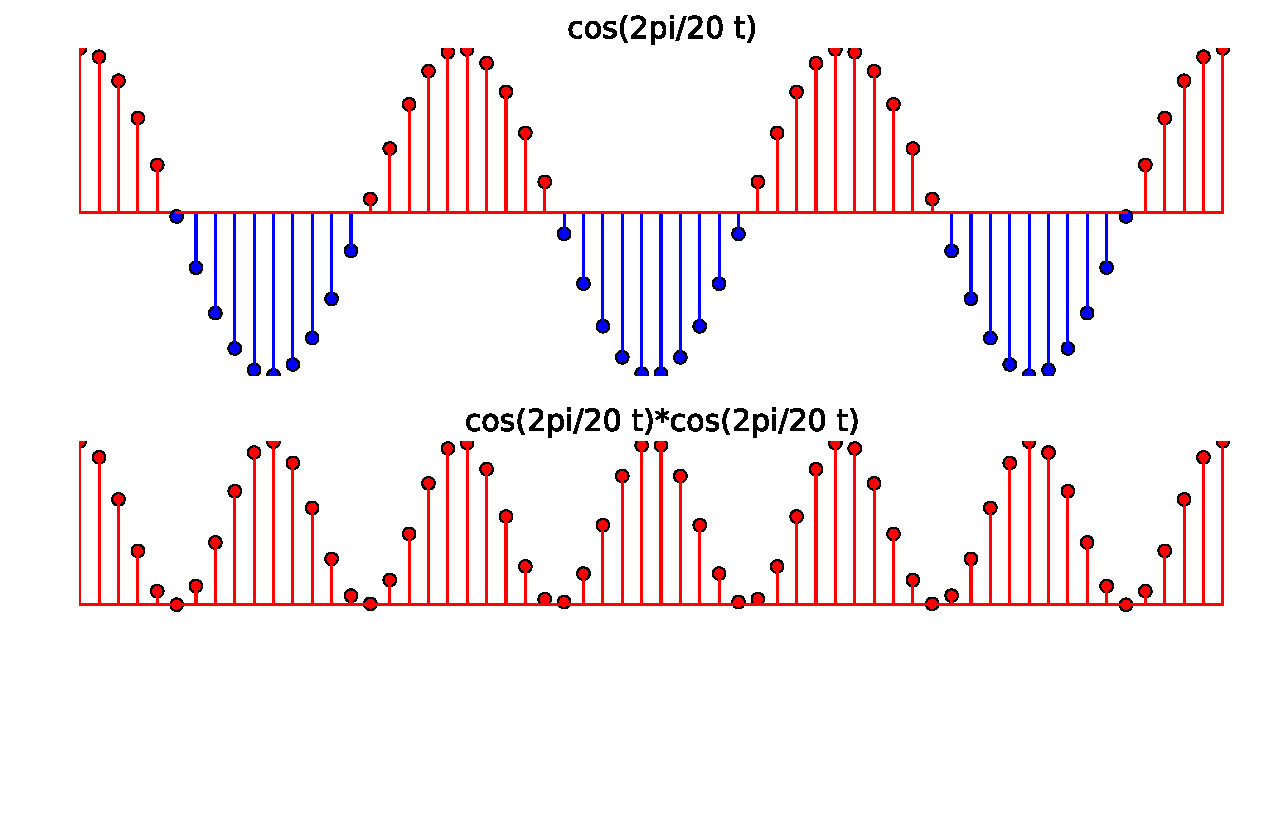
\includegraphics[width=\textwidth]{cosSqr.pdf}
\end{figure}

\end{frame}

\begin{frame}{Discrete Cosine Integration}

What is 

\[ \sum_{t=1}^{N=kT} \cos^2(\frac{2 \pi t}{T}) \]
?\\

Note that $\cos^2(A) = \frac{1 + \cos(2A)}{2}$

\end{frame}

\begin{frame}{Discrete Cosine Integration}

\begin{figure}[t]
    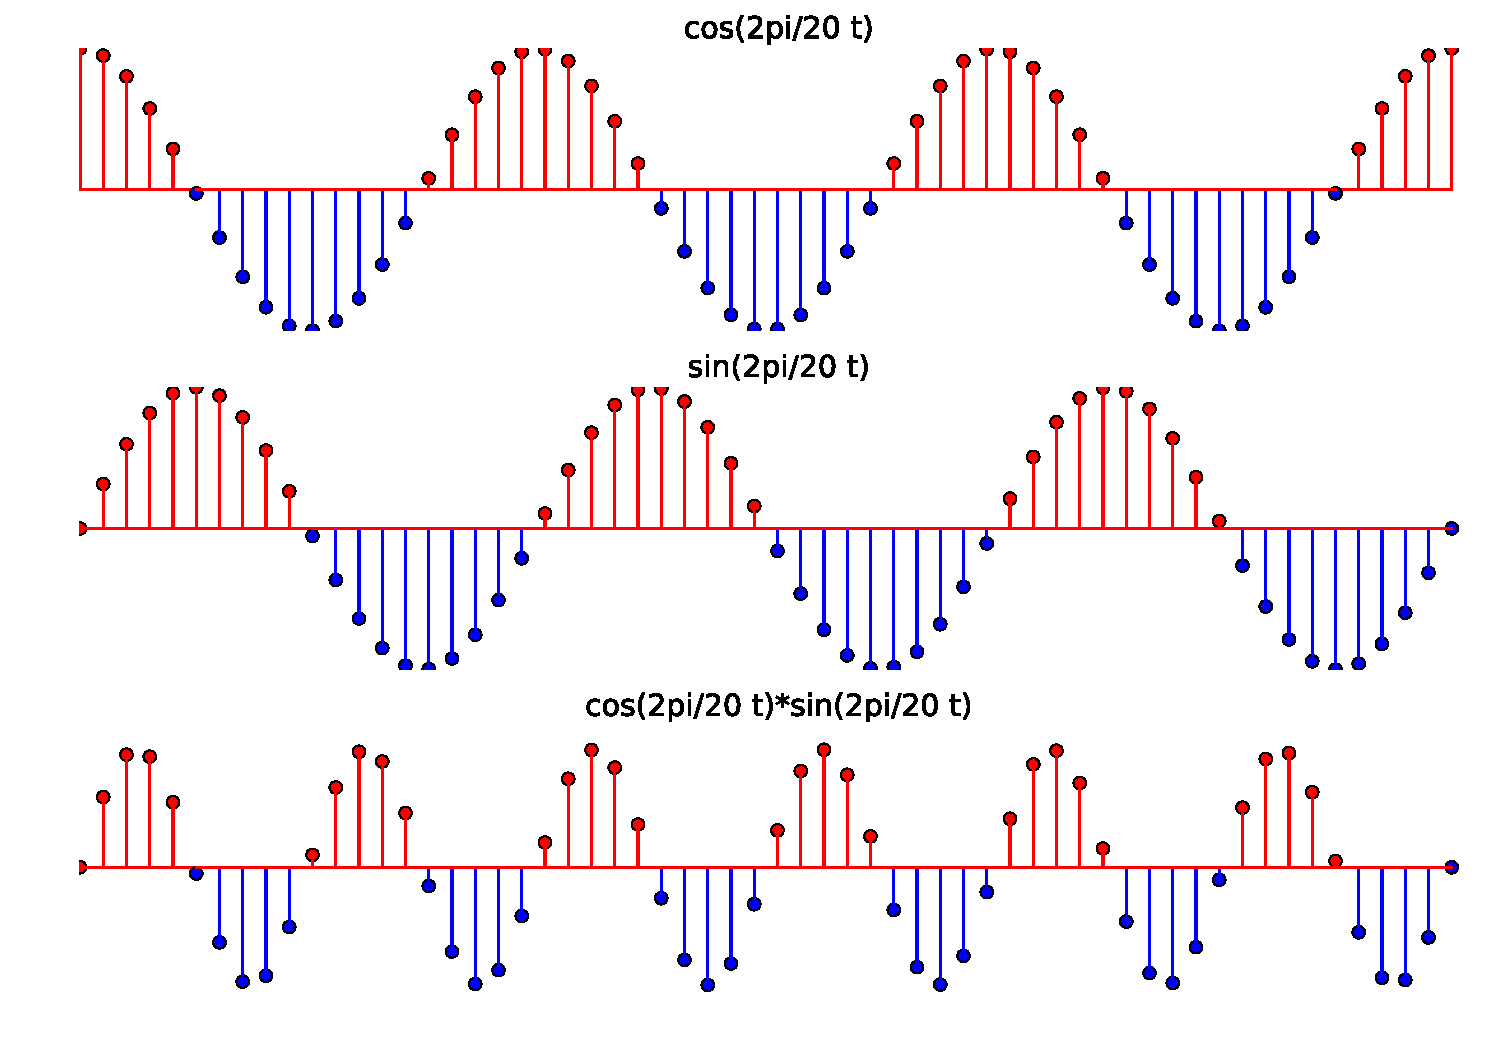
\includegraphics[width=\textwidth]{cossin.pdf}
\end{figure}

\end{frame}

\begin{frame}{Discrete Cosine Integration}

Why is $\sum_{t=1}^{N=kT} \cos(\frac{2 \pi t}{T}) \sin(\frac{2 \pi t}{T})$ zero?

Note that 

\[ \cos(A) \sin(A) = \frac{1}{2} \sin(2A) \]


\end{frame}

\begin{frame}{Discrete Cosine Integration}

\begin{figure}[t]
    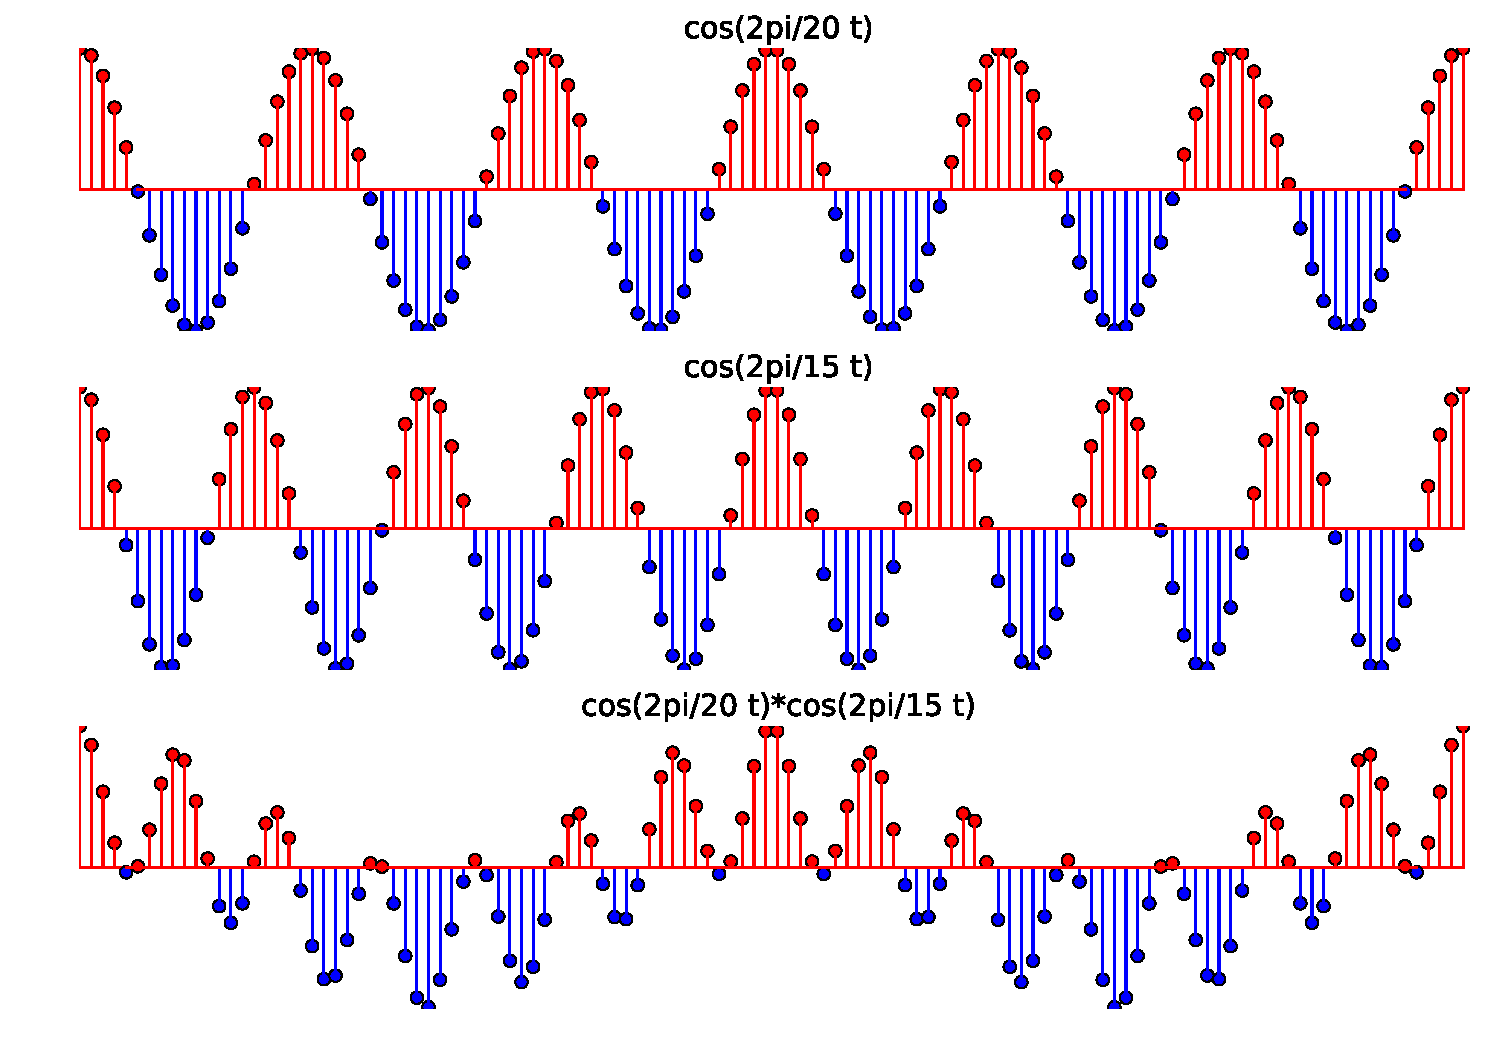
\includegraphics[width=\textwidth]{cosProd1.pdf}
\end{figure}

\end{frame}

\begin{frame}{Discrete Cosine Integration}

Why does the product of two different cosines integrate to zero?

\[ \cos(A+B) = \cos(A)\cos(B) - \sin(A)\sin(B) \]

\uncover<2->{
\[ \text{Hint:} \cos(A+B) + \cos(A-B) = ? \]
}

\end{frame}

\begin{frame}{Discrete Cosine Integration}

\begin{figure}[t]
    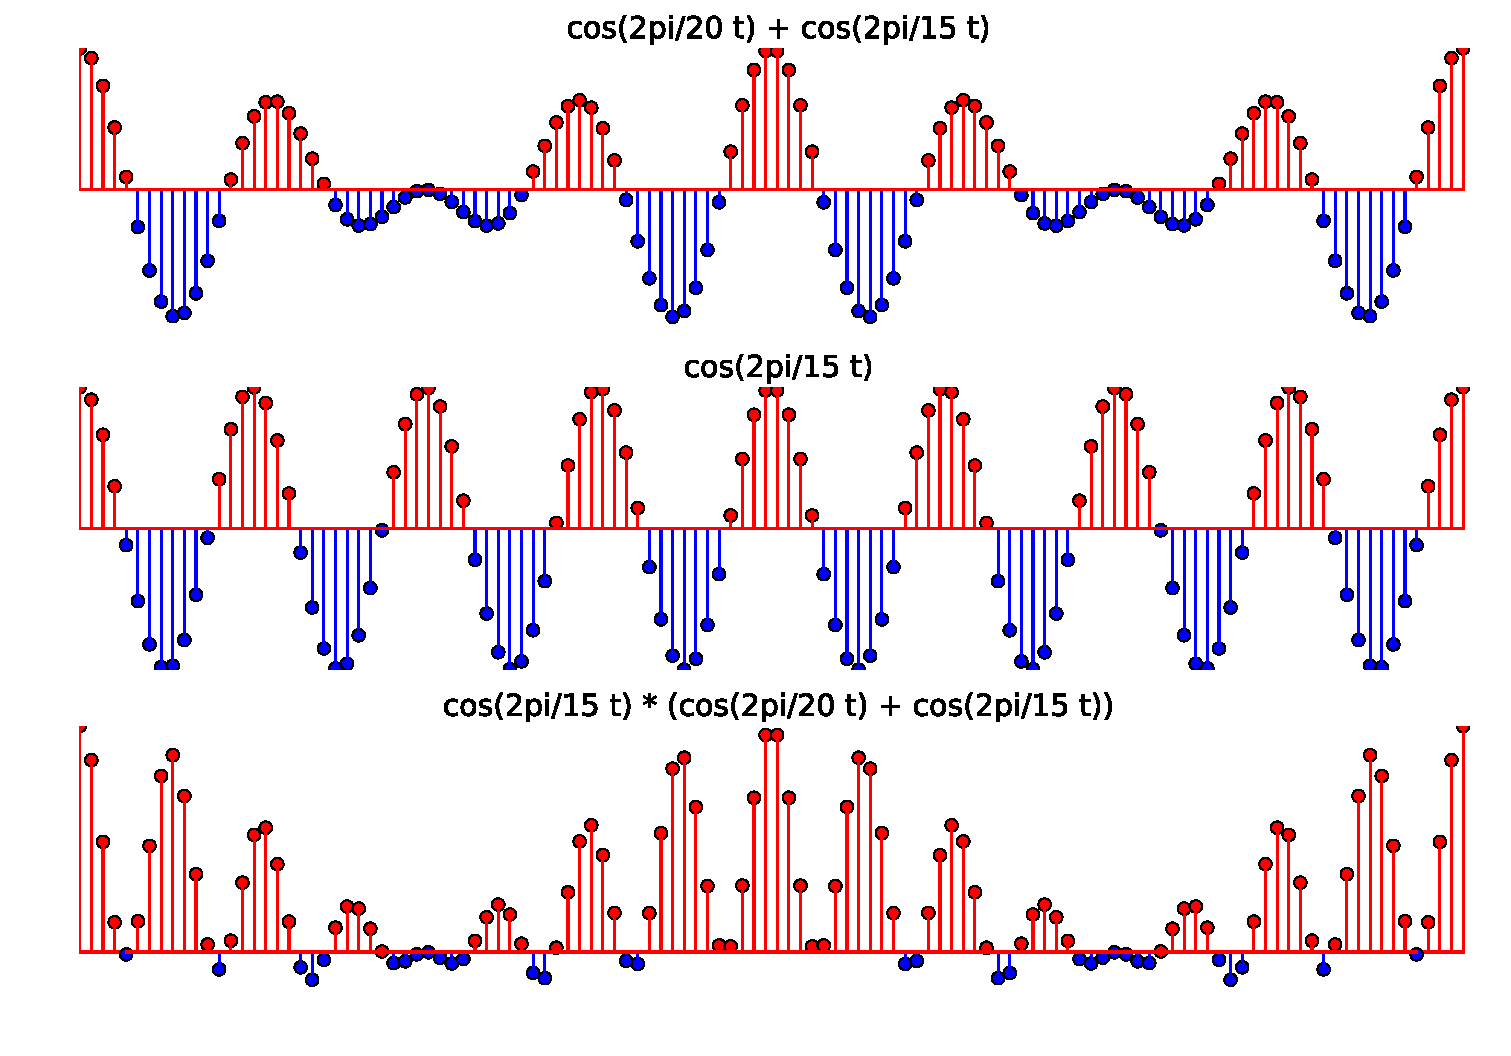
\includegraphics[width=\textwidth]{cosProd2.pdf}
\end{figure}

\end{frame}

\begin{frame}{Discrete Cosine Integration}

Dot product interpretation

\[ \vec{s_1} = \left[ 1, \cos\left( \frac{2 \pi}{T_1} \right), \cos\left( \frac{2 \pi 2}{T_1} \right) \hdots, \cos\left( \frac{2 \pi N}{T_1} \right) \right] \]

\[ \vec{s_2} = \left[ 1, \cos\left( \frac{2 \pi}{T_2} \right), \cos\left( \frac{2 \pi 2}{T_2} \right) \hdots, \cos\left( \frac{2 \pi N}{T_2} \right) \right] \]

Dot product is linear!

\[ \vec{s_2} \cdot (a\vec{s_1} + b\vec{s_2}) = a\vec{s_1} \cdot \vec{s_2} + b \vec{s_2} \cdot \vec{s_2} \]

Can use this type of dot product / integration to detect / test for the presence of different frequencies

\end{frame}

\begin{frame}{Cosine Phase Separation}

The general form of a sinusoid is $A\cos(\omega t + \phi)$

\[ A \cos(\omega t + \phi) = A\cos(\phi)\cos(\omega t) - A\sin(\phi)\sin(\omega t) \]

\uncover<2->{
\[ \cos(\omega t) (A \cos(\omega t + \phi) ) = A\cos(\phi)\cos^2(\omega t) - A\cos(\omega t)\sin(\phi)\sin(\omega t) \]
}

\begin{itemize}[label=$\vartriangleright$]
\uncover<3->{
\item The ``cosine component" of the sinusoid is $A \cos(\phi)$
\item The ``sinusoid component" of the sinusoid is $A \sin(\phi)$
}
\uncover<4->{
\item The {\em magnitude} $A$ of this sinusoid is $\sqrt{(A \cos(\phi))^2 + (A \sin(\phi))^2} = A$ (sanity check)
}
\end{itemize}

\end{frame}


\begin{frame}{Sinusoidal Coordinates \ Basis}

\tiny For a signal of length $N$ (let $N$ be odd for the moment), define the following matrix

\tiny
\[ F = \left[ \begin{array}{ccccc} 1 & 1 & 1 & \hdots & 1 \\ 1 & \cos(\frac{2\pi}{N}) & \cos(2\frac{2\pi}{N}) & \hdots & \cos((N-1)\frac{2\pi}{N})   \\ 0 & \sin(\frac{2\pi}{N}) & \sin(2\frac{2\pi}{N}) & \hdots & \sin((N-1)\frac{2\pi}{N}) \\ 

1 & \cos(\frac{4\pi}{N}) & \cos(2\frac{4\pi}{N}) & \hdots & \cos((N-1)\frac{4\pi}{N})   \\ 0 & \sin(\frac{4\pi}{N}) & \sin(2\frac{4\pi}{N}) & \hdots & \sin((N-1)\frac{4\pi}{N})

\\ \vdots & \vdots & \vdots & \hdots & \vdots \\

1 & \cos(\frac{((N-1)\pi}{N}) & \cos(2\frac{(N-1)\pi}{N}) & \hdots & \cos((N-1)\frac{(N-1)\pi}{N})   \\ 0 & \sin(\frac{(N-1)\pi}{N}) & \sin(2\frac{(N-1)\pi}{N}) & \hdots & \sin((N-1)\frac{(N-1)\pi}{N})


    \end{array} \right] \]

\begin{figure}[t]
    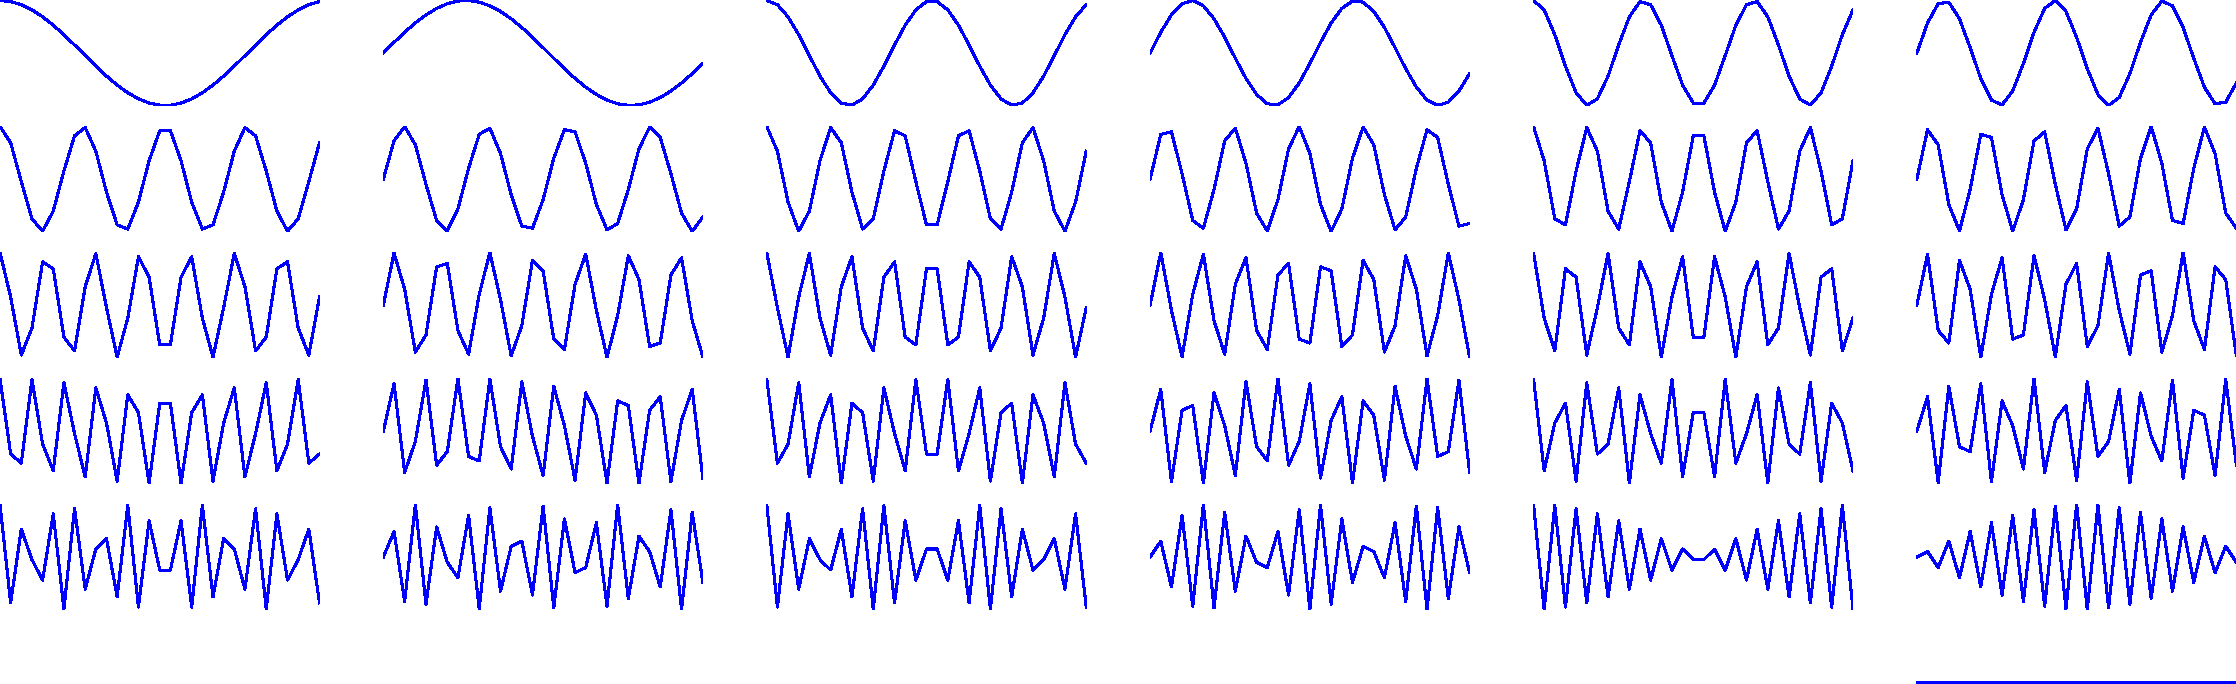
\includegraphics[width=\textwidth]{FourierBasis.pdf}
\end{figure}

\end{frame}


\begin{frame}

Each row is perpendicular to each other row.  This means that

\[ Fx \]

Is a high dimensional rotation!  This means these sinusoids form a \em{basis} for all signals of length $N$.  This is known as the {\em Discrete Fourier Transform}

\end{frame}

\begin{frame}{Discrete Fourier Transform: Example}

\begin{figure}[t]
    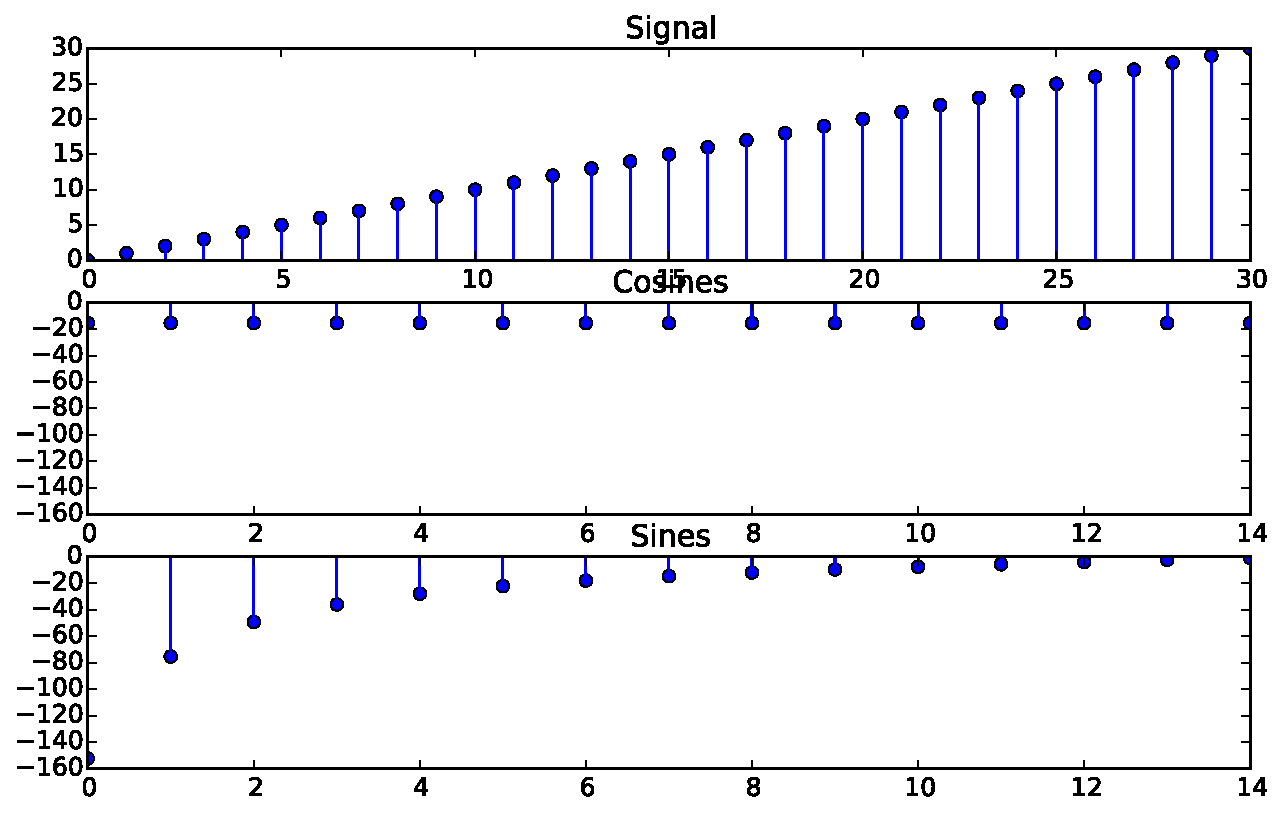
\includegraphics[width=\textwidth]{SawtoothWave.pdf}
\end{figure}

Show sinusoidal addition

\end{frame}

\begin{frame}{Discrete Fourier Transform: Example}

\begin{figure}[t]
    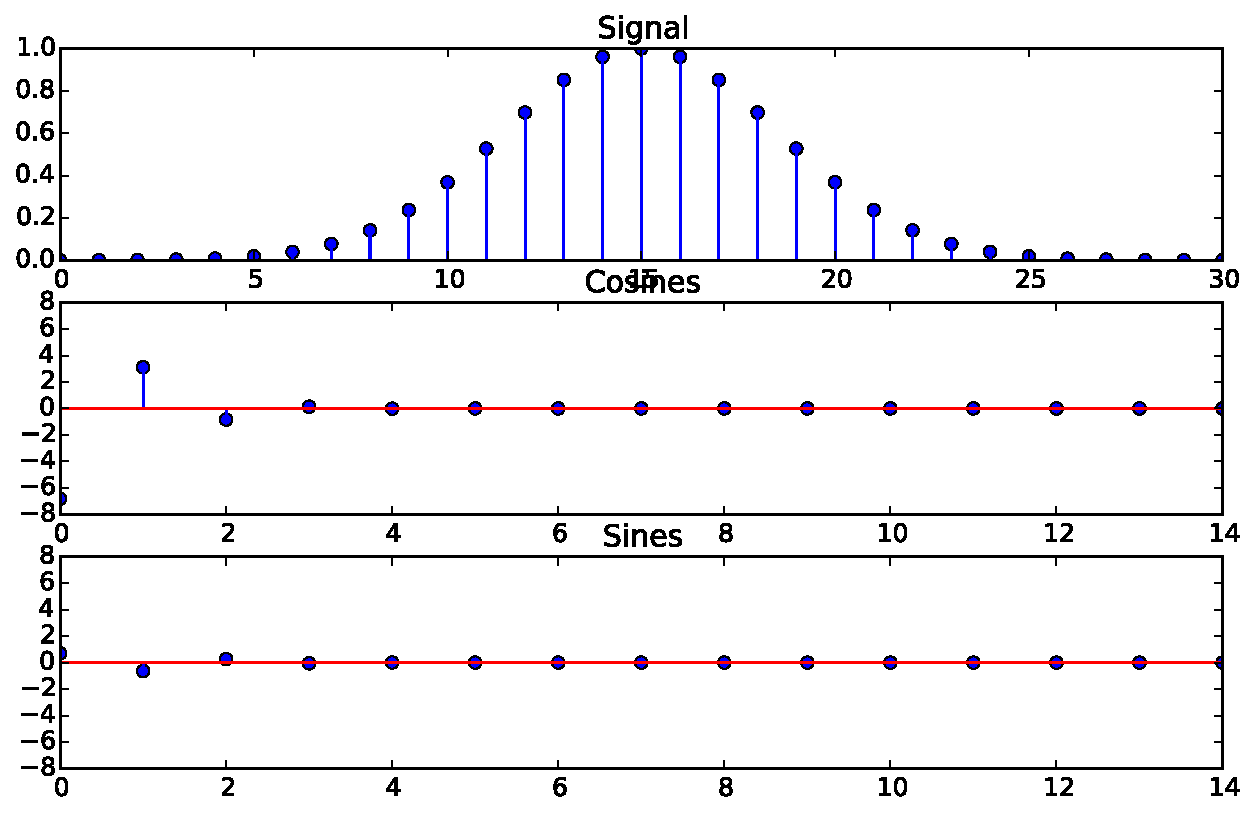
\includegraphics[width=\textwidth]{GaussianBump.pdf}
\end{figure}

Show sinusoidal addition
\end{frame}

\begin{frame}{Discrete Fourier Transform: Formal Definition}

The formal definition of the Discrete Fourier Transform uses complex numbers to store the phase, for convenience

\[ F[k] = \sum_{t = 0}^{N-1} X[n] e^{ -i 2 \pi \frac{k}{N} n } \]

\[ F[k] = \sum_{t = 0}^{N-1} X[n] \cos \left( 2 \pi \frac{k}{N} n \right) + i \sum_{t = 0}^{N-1} X[n] \sin \left( -2 \pi \frac{k}{N} n \right)  \]

\[ F[k] = \text{Re}(F[k]) + i \text{Imag}(F[k]) \]

\end{frame}

\begin{frame}{Inverse Discrete Fourier Transform}

DFT decomposed $X$ into a bunch of sinusoids, now add them back together

\[ X[n] = \sum_{k = 0}^{N-1} F[k] e^{i 2 \pi \frac{k}{N} n} \]

\end{frame}

\begin{frame}{Functions on The Circle}

\end{frame}

\end{document}

